\subsubsubsubsection{Street config reader}
\begin{figure}[h]
\centering
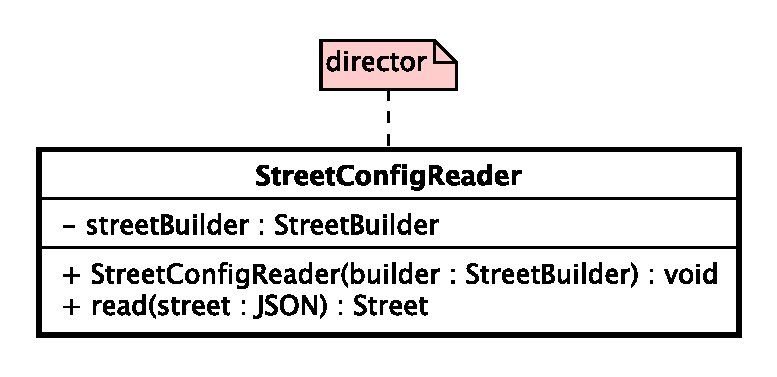
\includegraphics[scale=0.6,keepaspectratio]{images/solution/app/backend/street_config_reader.eps}
\caption{\pReactiveBuild::StreetConfigReader}
\label{fig:sd-app-street-config-reader}
\end{figure}
\FloatBarrier
\begin{itemize}
  \item \textbf{\descr} \\
    It represents the concrete director of the street builder.
    It has the responsibility to parse serializations of street.
  \item \textbf{\attrs}
  \begin{itemize}
    \item \texttt{builder: StreetBuilder} \\
The builder object which builds parts of the district.
  \end{itemize}
  \item \textbf{\ops}
  \begin{itemize} 
    \item[+] \texttt{StreetConfigReader(builder: StreetBuilder)} \\
Creates a concrete street director with its own street builder.
    \item[+] \texttt{read(street: JSON) : Street} \\
Parses a serialization of a street.
It uses the builder multiple times to create incrementally a 
specific configuration of the requested street specified 
in the configuration file. 
  \end{itemize}
\end{itemize}
